\documentclass[a4paper]{article}
\usepackage{global}
\headertext{中間報告}
\title{中間報告}
\author{
    由利大智
}
\date{}

\begin{document}

\maketitle

\begin{abstract}
P-core/E-coreが混在するヘテロジニアスNUMA環境では、スレッド配置によって性能が
大きく変動する。本研究では、局所性(通信コスト)とヘテロ性(コア性能差)を
単一の重み付き目的関数としてCP-SATで同時に最適化し、配置を決定するAKARIN
システムを提案する。当初検討していた固定戦略の分類予測から、配置そのものを
最適化するアプローチへと発展させた経緯、重みパラメータ$\alpha$の21点グリッド
探索とOptunaによるベイズ最適化を組み合わせた候補生成の設計、および実データに
よるパレート改善の確認について報告し、今後の定量評価に向けた進捗をまとめる。
\end{abstract}

\section{序論}
近年のCPUは、性能重視のP-core(Performance core)と電力効率重視のE-core(Efficiency core)
を組み合わせたヘテロジニアス構成が主流になりつつある。一方でコア数の増加に対して
メモリ帯域幅の増加は追いついておらず、さらに複数のNUMA(Non-Uniform Memory Access)
ノードにコアが分散配置されることで、スレッドをどのコアへ配置するかによって
メモリ帯域競合やノード間通信コストが大きく変動する。本研究では、Intel Core Ultra 9
285K(Arrow Lake)を模したヘテロジニアスNUMA環境を対象に、ワークロードごとに
最適なスレッド配置戦略が異なることに着目し、実行前に得られる特徴量から適切な配置を
決定する手法を検討している。

初期段階では、スレッドの割り当て順序を固定した4通りの静的戦略
(Packed/Scatter/HPO/EPO、詳細は3.1節)を比較対象とし、機械学習によってワークロード
特性から最適戦略を予測するアプローチを検討していた。しかし研究を進める中で、
固定戦略の組み合わせでは表現できない配置が実際には性能上優位であることが明らかになり、
現在はCP-SAT(制約充足・最適化ソルバ)を用いて、ワークロードごとに配置そのものを
最適化する\textbf{AKARINシステム}の設計・実装を中心に据えている(3節)。本報告では、
これまでの実験基盤の構築過程で得られた知見、AKARINシステムの現行設計、および評価に
向けた進捗を中間報告としてまとめる。

\section{関連研究}
本研究はJinによる修士論文\cite{jin}、およびその引用元であるAgung らのDeLoc\cite{deloc}
を主たる先行研究として参照している。DeLocは、実測したタスク間のメモリ通信量に基づいて
タスクペアを同一NUMAノードへ配置し(局所性)、ノード内では負荷の大きいタスクをBig
core、小さいタスクをSmall coreへ配分する(ヘテロ性)、という2段階のヒューリスティックで
MPO(Memory-congestion-aware Priority Option)を構成する。Jinの修士論文はこのMPOと、
P-core優先配置であるHPO(Heterogeneity-aware Priority Option)を、実測される通信量の
大小によってTabPFN等の分類器で切り替えるPOSM(Priority Option Switching Method)を
提案している。

本研究でも当初はPOSMとの比較を試みたが、DeLocが要求する実通信行列の取得には
Pinベースのトレーサ(detloc-tracer)が必要であり、開発環境のカーネルとの非互換により
当初は取得が困難であった。研究室が保有する著者ら本人の環境が現存する古いカーネルの
サーバを利用することで実データの取得には成功したものの、この過程でMPOが局所性と
ヘテロ性を2段階のヒューリスティックで独立に決定する設計であるため、ノード内のBig
core数を超える重いタスクは強制的にSmall coreへ落ちるという構造的な制約を持つことが
分かった。POSMはこのMPOとHPOのいずれかを選ぶ二値選択の枠組みであるため、
両者の中間的な配置や、局所性とヘテロ性を同時に満たす配置を表現できない。

この観察から、本研究では2段階ヒューリスティックによる戦略の選択ではなく、局所性
(ノード間通信コスト)とヘテロ性(コア性能差)を単一の目的関数として同時に最適化する
アプローチへと方向を転換した。これがAKARINシステムの設計思想であり、次節で詳細を
述べる。

\section{提案手法: AKARINシステム}

\subsection{4戦略の定義}
比較のベースラインとして、以下4通りのスレッド割り当て順序を用いる。いずれもNUMA
2ノード(各ノードにP-core 4個、E-core 4個)構成を前提とする。

\begin{itemize}
  \item \textbf{Packed}: 全スレッドをNode0から順に詰める(局所性重視)
  \item \textbf{Scatter}: 両ノードへ交互に分散させる(帯域分散重視)
  \item \textbf{HPO}: P-coreを優先して埋める(演算性能重視)
  \item \textbf{EPO}: E-coreを優先して埋める(電力効率重視)
\end{itemize}

\begin{figure}[t]
  \centering
  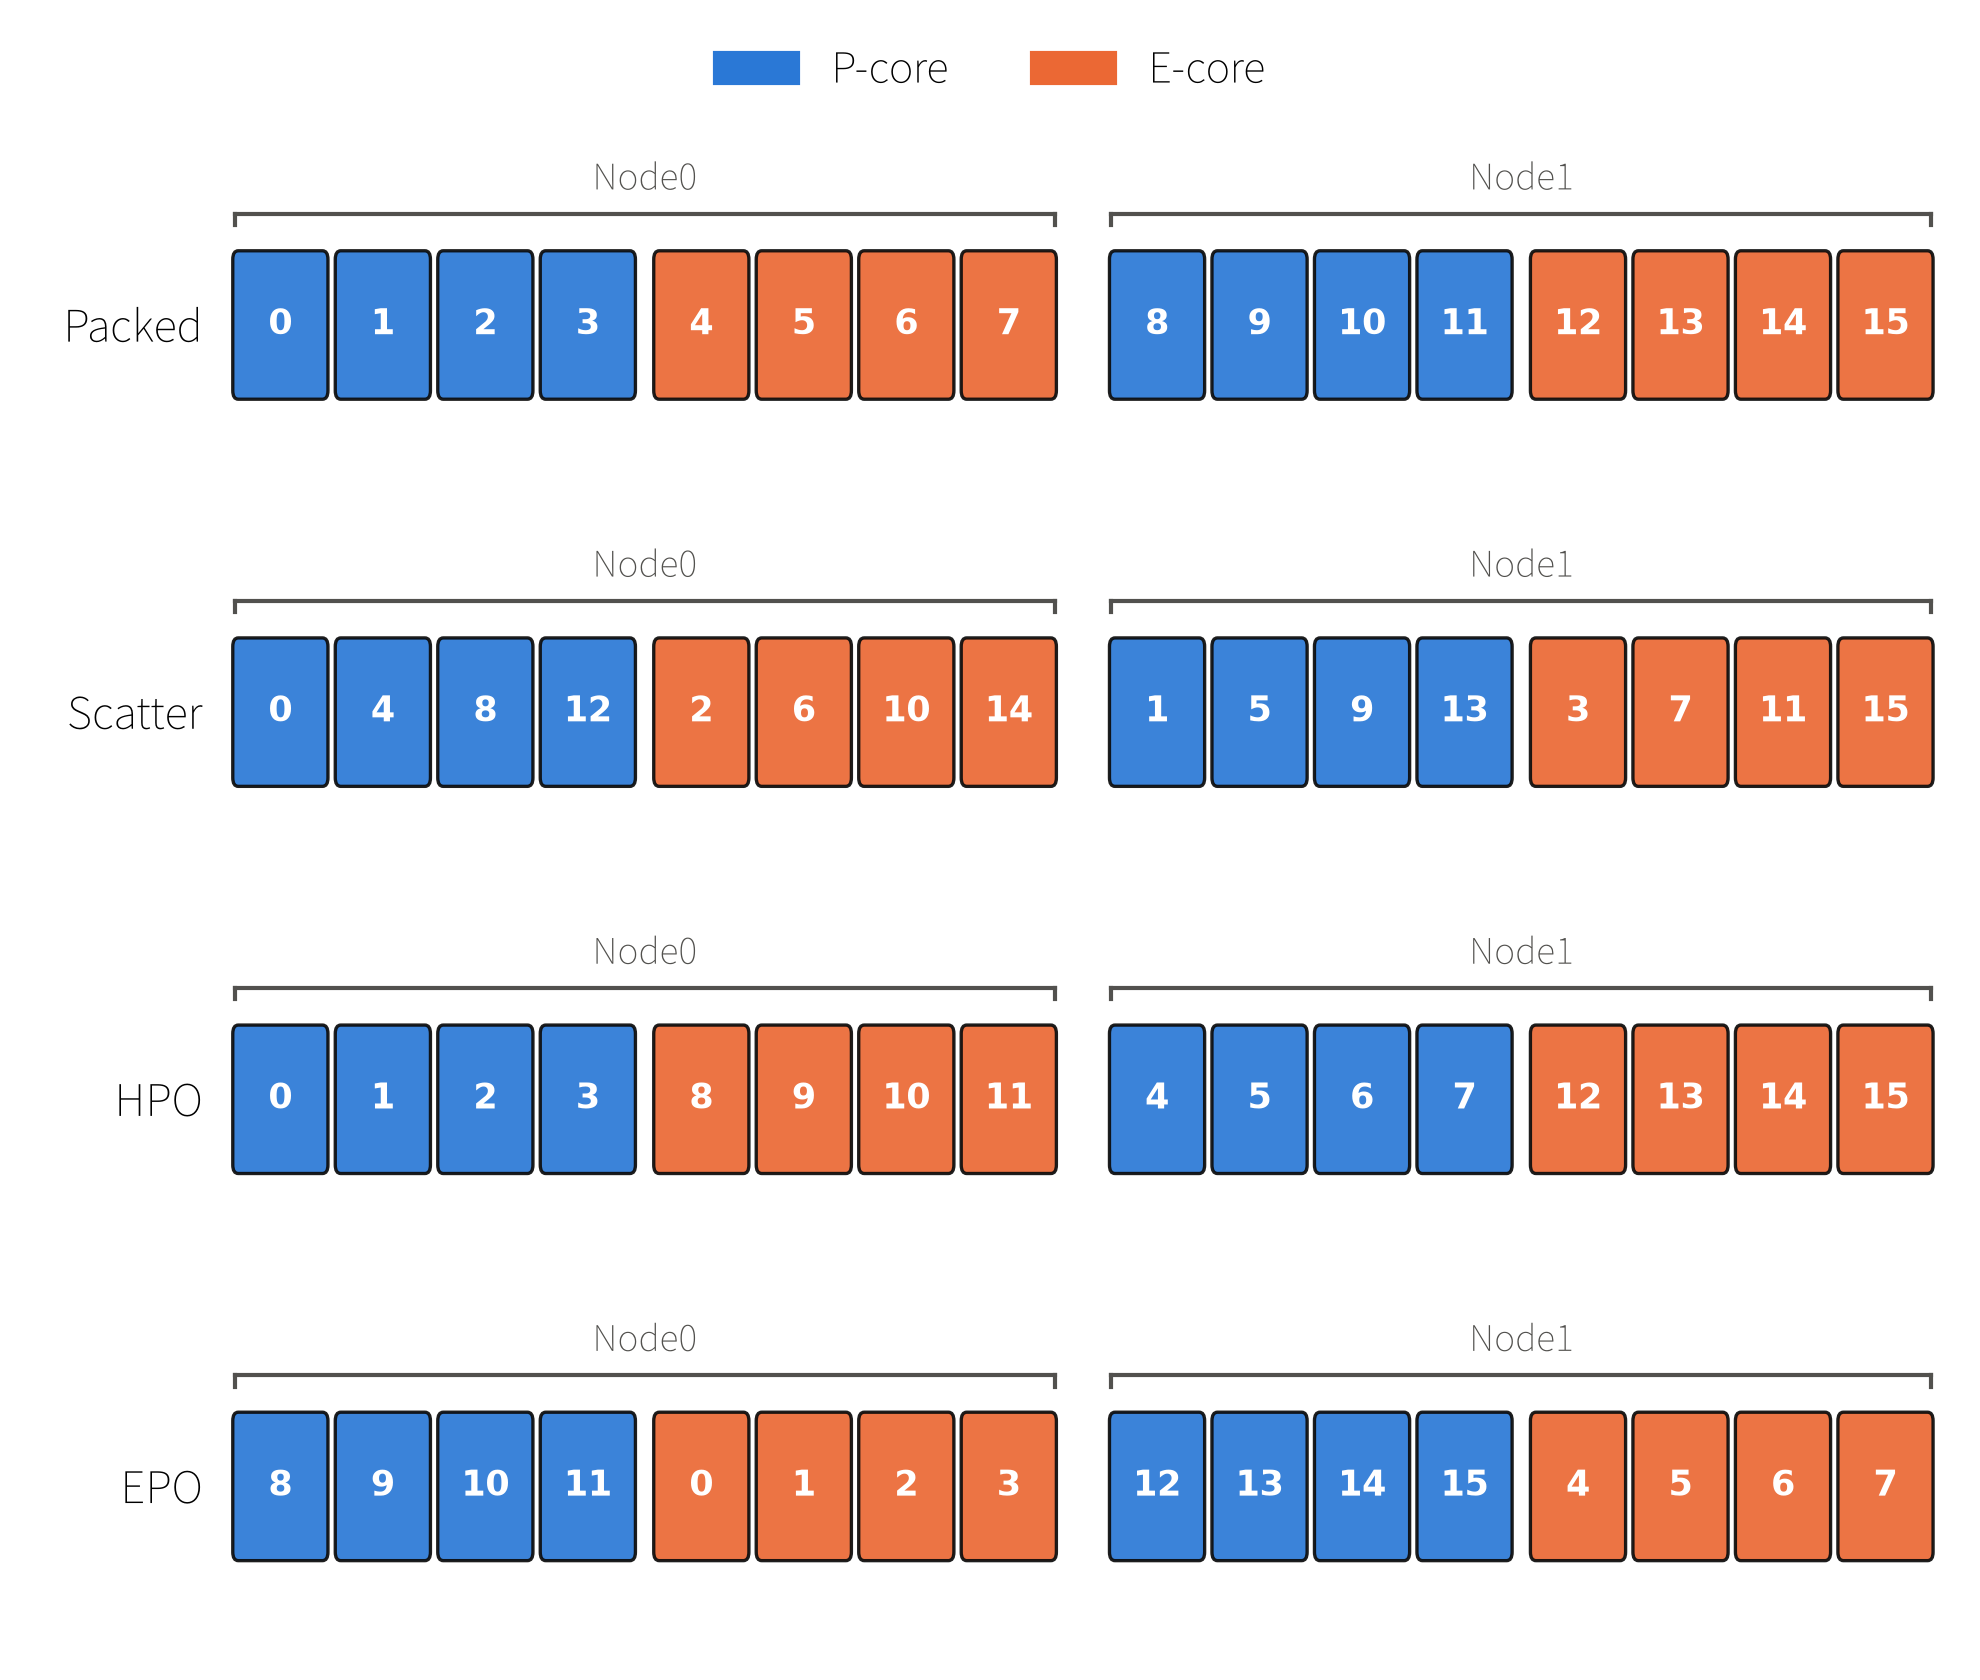
\includegraphics[width=\linewidth]{figs/strategies.png}
  \caption{16スレッド実行時の4戦略によるコア配置の比較。セル内の数値は
    そのコアに割り当てられるスレッド番号を示す。}
  \label{fig:strategies}
\end{figure}

図\ref{fig:strategies}に、16スレッド実行時の各戦略によるスレッド-コア対応を示す。

\subsection{目的関数: alpha加重によるCP-SAT最適化}
AKARINシステムでは、これら4戦略のような固定順序ではなく、各スレッドをどのコアへ
配置するかを決定変数として直接最適化する。局所性(ノード間通信コスト)とヘテロ性
(コア性能差)という2つの要因を、パラメータ$\alpha \in [0, 1]$による重み付き和として
単一の目的関数に統合する。

\begin{equation}
  \mathrm{cost} = \alpha \cdot \mathrm{makespan} + (1 - \alpha) \cdot \mathrm{remote\_penalty}
\end{equation}

ここで$\mathrm{makespan}$はノード内の各コアの完了時間の最大値であり、コア性能差
(P-core/E-coreの周波数差)によるヘテロ性を表現する。$\mathrm{remote\_penalty}$は
スレッド間の実測通信量(mem\_access.csv/comm\_size.csvから算出)のうち、異なる
NUMAノードをまたぐ通信に対するペナルティであり、局所性を表現する。$\alpha=1$は
速度(ヘテロ性)のみを重視した配置、$\alpha=0$は通信量(局所性)のみを重視した配置
に相当し、中間の$\alpha$は両者のトレードオフを取った配置となる。

\subsection{候補生成: alphaグリッド探索とOptunaによるベイズ最適化}
上記の目的関数を最小化するスレッド-コア割り当てを、Google OR-Toolsの制約プログラ
ミングソルバCP-SATで$\alpha$ごとに解く。$\alpha \in [0, 1]$を21等分した密グリッドで
候補cpu\_mapを生成し、それぞれについてSniperでフル実行して実測sim\_timeを取得する
パイプライン(\texttt{akarin/generate\_candidates.py})を構築した。当初はワークロードの
重量級/軽量級によってグリッドの粗密を使い分けていたが、Size Sクラスは相対的に
Sniper実行コストが低いため、現在は全ワークロードで21点の密グリッドに統一している。
さらに、グリッド探索を補完する形で、$\alpha$候補ごとにCP-SATでcpu\_mapを計算し
実際にSniperを実行、実測sim\_timeをOptunaへフィードバックするベイズ最適化(TPE)
ループ(\texttt{akarin/optuna\_search.py})も実装した。

\begin{figure}[t]
  \centering
  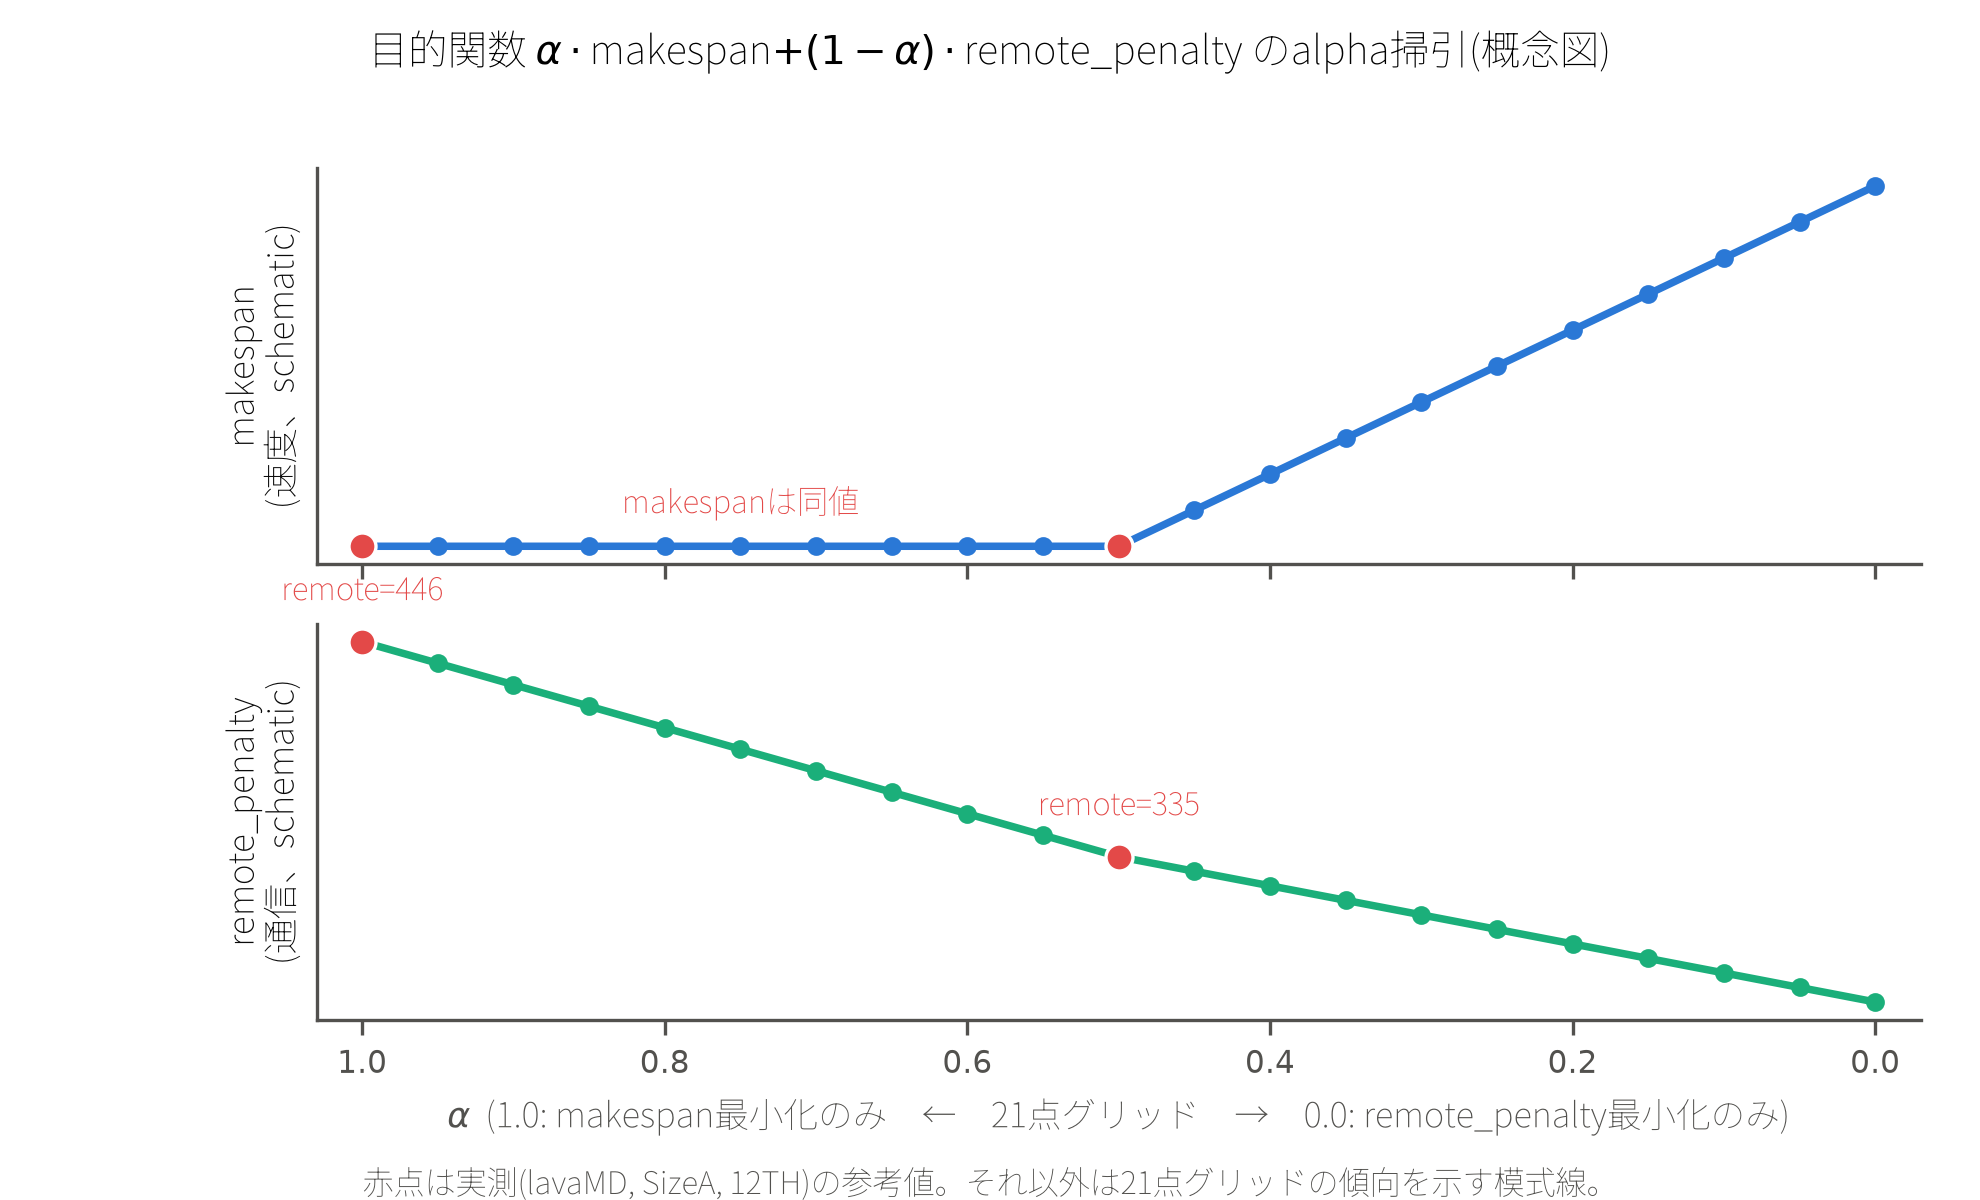
\includegraphics[width=\linewidth]{figs/alpha_sweep.png}
  \caption{$\alpha$を21点グリッドで掃引した場合のmakespan/remote\_penaltyの
    概念図。赤点はlavaMD(SizeA、12TH)での実測を示す参考点で、$\alpha=1.0$と
    $\alpha=0.5$は同一のmakespanを保ちながらremote\_penaltyが446から335へ改善する
    パレート改善を確認している。}
  \label{fig:alpha_sweep}
\end{figure}

図\ref{fig:alpha_sweep}にlavaMD(SizeA、12TH)での実測例を示す。$\alpha=0.5$は
$\alpha=1.0$と同じ最良makespanを保ちながら通信ペナルティも改善するパレート改善を
確認しており、DeLocの2段階ヒューリスティックがノード制約によって構造的に見逃す
配置を、CP-SATによる同時最適化が捉えられることを示唆している。

\subsection{今後の学習ベースアプローチとの統合}
本研究の主眼は「AIによる自動最適化」であり、DeLocのようなルールベース手法を
未知のワークロードへの汎化性の弱さの観点から批判する立場にある。そのため、
$\alpha$という重み自体を人手で調整するのではなく、TabPFN等の学習モデルに
ワークロードの生の特徴量を渡し、実測sim\_timeやパレート最適な$\alpha$を直接
予測させる方向への統合を今後の方針として検討している。

\section{実験環境}

\subsection{シミュレータの選定}
本研究では当初アーキテクチャシミュレータgem5を用いていたが、O3CPUモデルでNPB
BenchmarkのClass A(16スレッド)を実行するのに約30日を要すると実測から見積もられ、
実験規模の確保が困難と判断した。Sniperはinterval simulationとPINベースの動的計装を
採用しており、gem5比で10〜100倍高速に実行できるため、本研究の後半からはSniperへ
全面移行している。

\subsection{ハードウェアモデル}
評価対象はIntel Core Ultra 9 285K(Arrow Lake)を模したNUMA 2ノード構成である。
各ノードにP-core 4個・E-core 4個(計16コア)を配置し、ノードごとに独立したDRAM
コントローラ(実効帯域51.2\,GB/s)を持たせ、ノード間はバスモデル(共有帯域
102.4\,GB/s)で接続する。

\subsection{ワークロード}
NPB(NAS Parallel Benchmarks)からBT/FT/IS/MG、PARSECからcanneal/dedup、
加えてランダムメモリアクセスを行う合成ベンチマークGUPSの計7種類を評価対象と
している。GAPBS系グラフベンチマーク(BFS/PR/BC/CC/SSSP/TC)、lavaMD、
fluidanimate、water\_nsquaredは、pthread/OpenMPの同期プリミティブに起因する
Sniper本体のfutexデッドロック(6節参照)により除外した。x264はPARSEC同梱版が
フレームごとに使い捨てpthreadを生成する設計であり、「指定したスレッド数を
固定でNUMA配置する」という本研究の前提と根本的に噛み合わないため対象外とした。

\section{評価}
評価パイプラインは、事前計測した特徴量から最適なスレッド配置戦略(あるいは
AKARINによる動的配置)を予測する複数のモデル(Random Forest、SVM、XGBoost、
TabPFN)を比較する構成である。4戦略に加えてAKARIN候補を5クラス目として含めた
比較を実施したところ、以下の結果を得た。

\begin{table}[h]
  \centering
  \small
  \begin{tabular}{lcc}
    \toprule
    モデル & 4クラス($n{=}23$) & 5クラス AKARIN込み($n{=}31$) \\
    \midrule
    RF     & 0.609 & 0.516 \\
    SVM    & 0.435 & 0.516 \\
    XGB    & 0.609 & 0.581 \\
    TabPFN & ---   & 0.548 \\
    \bottomrule
  \end{tabular}
  \caption{4クラス(既存戦略のみ)と5クラス(AKARIN込み)の分類精度比較。}
  \label{tab:akarin_comparison}
\end{table}

31サンプル中4件(約13\%)でAKARINが実際に最良の戦略として選ばれており、クラス数
増加に伴って単純な分類精度は総じて低下したものの、これは既存4戦略だけでは
取りこぼしていたケースをAKARINが拾えていることの裏返しでもある。ただし
サンプル数(31件)は理論上の最大値に対して大幅に少なく、AKARIN実行データの
不足やスレッド数構成の過渡的な変更などが原因である。今後はデータ収集を進め、
より大きなサンプルサイズでの再評価が必要である。

\section{考察}
現時点で残る未解決の課題として、以下2点が挙げられる。

\textbf{Sniper本体のfutexデッドロック}: pthreadの同期プリミティブ(mutex/condition
variable/barrier)を多用するワークロードにおいて、シミュレータのリプレイエンジンが
記録時のスレッド間happens-before関係を保証できないことに起因すると考えられる
確率的なデッドロックを確認している。原因の層(SIFTトレース形式がスレッド間の
順序情報を保持しない設計であること)は特定できたが、根本修正にはシミュレータの
コア部分の再設計が必要でリスクが大きいため、該当するワークロード(water\_nsquared、
BFS/PR等のGAPBS系)を評価対象から除外する対応に留めている。

\textbf{非対称NUMAトポロジのモデリング}: 本研究が対象とするアーキテクチャは、
1つのNUMAノード内にP-coreとE-coreが混在するという、一般的なソケット単位のNUMA
(ノード内は同種コア)とは異なる構成である。現行のNUMAモデルがこの非対称性を
どこまで忠実に表現できているかは検証途上であり、今後の課題としたい。

\section{今後の課題}
\begin{itemize}
  \item AKARIN実行データの収集を進め、より大きなサンプルサイズでモデル比較を
    再評価する
  \item $\alpha$の選択自体を人手のグリッド探索に委ねるのではなく、TabPFN等の
    学習モデルにワークロード特性から直接予測させる方向を検証する
  \item $\mathrm{makespan}$項が計算時間のみを見ており、同一ノード内での帯域競合
    (輻輳)によるメモリアクセス待ち時間を捉えられていない点の精緻化を検討する
  \item 非対称NUMAトポロジ(1ノード内のP/E-core混在)のモデリング精度を検証する
  \item futexデッドロックにより除外しているワークロード群について、タイムアウト
    検知・再試行等の安全弁による対象復帰の可否を検討する
\end{itemize}

\section{まとめ}
本報告では、ヘテロジニアスNUMA環境におけるスレッド配置最適化を目的とした本研究の
これまでの進捗をまとめた。当初検討していた固定戦略の分類予測というアプローチから、
局所性とヘテロ性を単一の重み付き目的関数($\alpha \cdot \mathrm{makespan} +
(1-\alpha) \cdot \mathrm{remote\_penalty}$)としてCP-SATで同時に最適化する
AKARINシステムへと設計を発展させ、21点の$\alpha$グリッド探索とOptunaによる
ベイズ最適化ループを実装した。実データによる検証(lavaMD、SizeA、12TH)では、
$\alpha$の選び方によって同一のmakespanを保ちながら通信ペナルティを改善する
パレート改善が得られることを確認し、AKARIN候補を含めた5クラスのモデル比較でも
一定の割合でAKARINが最良戦略として選択されることを確認した。今後は、データ収集を
拡充した上で定量的な比較評価を進めていく。

\begin{thebibliography}{9}
\bibitem{jin} Yifan Jin (指導: 滝沢寛之), ``Memory-aware Task Mapping for
  Heterogeneous Multi-Core Systems,'' Master's Thesis, Graduate School of
  Information Sciences, Tohoku University, Jan.\ 2022.
\bibitem{deloc} M. Agung, M. A. Amrizal, R. Egawa, and H. Takizawa,
  ``DeLoc: A Locality and Memory-Congestion-Aware Task Mapping Method for
  Modern NUMA Systems,'' IEEE Access, vol.\,8, pp.\,6937--6953, 2020,
  doi: 10.1109/ACCESS.2019.2963726.
\end{thebibliography}

\end{document}
